\section{Compilatie vs Interpretatie}

\frame{\tableofcontents[currentsection]}

\begin{frame}
  \frametitle{Taal van de CPU}
  \begin{center}
    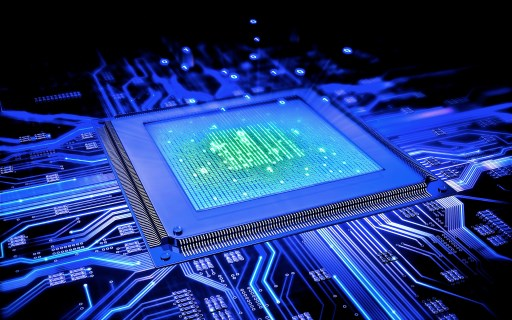
\includegraphics[width=5cm]{cpu.jpg}
  \end{center}
  \begin{itemize}
    \item CPU begrijpt enkel machinecode
    \item CPU kan instructies in machinecode razendsnel uitvoeren
    \item Hel voor de mens om in te programmeren
  \end{itemize}
\end{frame}

\begin{frame}
  \frametitle{Programmeertalen}
  \begin{itemize}
    \item Talen ontwikkeld om het de mens gemakkelijker te maken
    \item Bv.~oudste taal: FORTRAN (Formula Translator)
  \end{itemize}
  \begin{center}
    \begin{tikzpicture}[code/.style={draw,drop shadow,fill=white}]
      \node[code,font=\small] (asm) at (0,0) {
        \parbox{6cm}{
          \code[width=\linewidth,frame=none]{addition.asm}
        }
      };
      \node[anchor=west,code,font=\small] (cpp) at ($ (asm.east) + (1,0) $) {
        \ttfamily\small z = x + y
      };
      \draw[-latex] (asm.east) -- (cpp.west);
    \end{tikzpicture}
  \end{center}
\end{frame}

\begin{frame}
  \frametitle{Vertaling}
  \begin{itemize}
    \item Programmeertaal moet vertaald worden naar machinecode
    \item Spectrum aan verschillende technieken mogelijk
    \item Uiteindes: compilatie en interpretatie
  \end{itemize}
  \begin{center}
    \begin{tikzpicture}[approach/.style={drop shadow,rotate=90,minimum width=3cm,minimum height=1cm},
                        language/.style={font=\tiny,minimum width=1.8cm,minimum height=.5cm,rotate=90,opacity=0.25,draw,text opacity=1,fill=white}]
      \node[approach,fill=green!50] (compilation) at (-4,0) {Compilatie};
      \path[left color=green!50,right color=red!50,drop shadow] (-3.5,-1) rectangle (3.5,1);
      \node[approach,fill=red!50] (interpretation) at (4,0) {Interpretatie};
      \node[language] (cpp) at (-3,0) {C++};
      \node[language] (python) at (2,0) {Python};
      \node[language] (ruby) at (3,0) {Ruby};
      \node[language] (java) at (-1,0) {Java};
      \node[language] (csharp) at (-2,0) {C$^\sharp$};
      \node[language] (javascript) at (1,0) {JavaScript};
      \node[language] (lisp) at (0,0) {Common Lisp};
    \end{tikzpicture}
  \end{center}
\end{frame}

\subsection{Compilatie}

\frame{\tableofcontents[currentsubsection]}

\begin{frame}
  \frametitle{Compilatie: Analogie}
  \begin{itemize}
    \item Je bent kok
    \item Je spreekt enkel Nederlands
    \item Je krijgt een keukenrecept
    \item Oorspronkelijk was het recept in het Japans
    \item Gelukkig werd het op voorhand vertaald
    \item Er werd rekening gehouden met je eigen keukeninrichting
    \item Je kan er dus effici\"ent mee overweg
  \end{itemize}
\end{frame}

\begin{frame}
  \frametitle{Compilatie}
  \structure{Voordelen}
  \begin{itemize}
    \item Code wordt effici\"ent uitgevoerd
    \item Compilatie checkt op fouten
  \end{itemize}
  \vskip5mm
  \structure{Nadelen}
  \begin{itemize}
    \item Alle code moet op voorhand beschikbaar zijn
    \item Code genereren at runtime gaat niet
    \item Code kan niet aangepast worden tijdens uitvoering
    \item Hercompilatie nodig bij wijziging code
  \end{itemize}
\end{frame}

\subsection{Interpretatie}

\frame{\tableofcontents[currentsubsection]}

\begin{frame}
  \frametitle{Compilatie: Analogie}
  \begin{itemize}
    \item Je bent kok
    \item Je spreekt enkel Nederlands
    \item Je krijgt een keukenrecept
    \item Het recept is in het Japans
    \item Je krijgt een woordenboek en grammaticaboek
    \item 't Koken gaat wat minder effici\"ent gebeuren
  \end{itemize}
\end{frame}

\begin{frame}
  \frametitle{Interpretatie}
  \structure{Voordelen}
  \begin{itemize}
    \item Nieuwe code kan tijdens uitvoering geproduceerd worden
    \item Code kan aangepast worden tijdens uitvoering
    \item Meer flexibiliteit in het algemeen
  \end{itemize}
  \vskip5mm
  \structure{Nadelen}
  \begin{itemize}
    \item Code kan nog allerhande typfouten bevatten die pas tijdens uitvoering worden opgemerkt
    \item Code werkt veel trager omdat het ter plekke nog vertaald moet worden
  \end{itemize}
\end{frame}

\subsection{Python}

\frame{\tableofcontents[currentsubsection]}

\begin{frame}
  \frametitle{Python}
  \begin{itemize}
    \item Python is hybride
    \item Neigt eerder naar interpretatie kant
    \item Python staat niet gekend voor snelheid
    \item Python geeft wel heel wat vrijheid eigen aan interpretatie
  \end{itemize}
\end{frame}


%%% Local Variables:
%%% mode: latex
%%% TeX-master: "python"
%%% End:
